\documentclass[1p]{elsarticle_modified}
%\bibliographystyle{elsarticle-num}

%\usepackage[colorlinks]{hyperref}
%\usepackage{abbrmath_seonhwa} %\Abb, \Ascr, \Acal ,\Abf, \Afrak
\usepackage{amsfonts}
\usepackage{amssymb}
\usepackage{amsmath}
\usepackage{amsthm}
\usepackage{scalefnt}
\usepackage{amsbsy}
\usepackage{kotex}
\usepackage{caption}
\usepackage{subfig}
\usepackage{color}
\usepackage{graphicx}
\usepackage{xcolor} %% white, black, red, green, blue, cyan, magenta, yellow
\usepackage{float}
\usepackage{setspace}
\usepackage{hyperref}

\usepackage{tikz}
\usetikzlibrary{arrows}

\usepackage{multirow}
\usepackage{array} % fixed length table
\usepackage{hhline}

%%%%%%%%%%%%%%%%%%%%%
\makeatletter
\renewcommand*\env@matrix[1][\arraystretch]{%
	\edef\arraystretch{#1}%
	\hskip -\arraycolsep
	\let\@ifnextchar\new@ifnextchar
	\array{*\c@MaxMatrixCols c}}
\makeatother %https://tex.stackexchange.com/questions/14071/how-can-i-increase-the-line-spacing-in-a-matrix
%%%%%%%%%%%%%%%

\usepackage[normalem]{ulem}

\newcommand{\msout}[1]{\ifmmode\text{\sout{\ensuremath{#1}}}\else\sout{#1}\fi}
%SOURCE: \msout is \stkout macro in https://tex.stackexchange.com/questions/20609/strikeout-in-math-mode

\newcommand{\cancel}[1]{
	\ifmmode
	{\color{red}\msout{#1}}
	\else
	{\color{red}\sout{#1}}
	\fi
}

\newcommand{\add}[1]{
	{\color{blue}\uwave{#1}}
}

\newcommand{\replace}[2]{
	\ifmmode
	{\color{red}\msout{#1}}{\color{blue}\uwave{#2}}
	\else
	{\color{red}\sout{#1}}{\color{blue}\uwave{#2}}
	\fi
}

\newcommand{\Sol}{\mathcal{S}} %segment
\newcommand{\D}{D} %diagram
\newcommand{\A}{\mathcal{A}} %arc


%%%%%%%%%%%%%%%%%%%%%%%%%%%%%5 test

\def\sl{\operatorname{\textup{SL}}(2,\Cbb)}
\def\psl{\operatorname{\textup{PSL}}(2,\Cbb)}
\def\quan{\mkern 1mu \triangleright \mkern 1mu}

\theoremstyle{definition}
\newtheorem{thm}{Theorem}[section]
\newtheorem{prop}[thm]{Proposition}
\newtheorem{lem}[thm]{Lemma}
\newtheorem{ques}[thm]{Question}
\newtheorem{cor}[thm]{Corollary}
\newtheorem{defn}[thm]{Definition}
\newtheorem{exam}[thm]{Example}
\newtheorem{rmk}[thm]{Remark}
\newtheorem{alg}[thm]{Algorithm}

\newcommand{\I}{\sqrt{-1}}
\begin{document}

%\begin{frontmatter}
%
%\title{Boundary parabolic representations of knots up to 8 crossings}
%
%%% Group authors per affiliation:
%\author{Yunhi Cho} 
%\address{Department of Mathematics, University of Seoul, Seoul, Korea}
%\ead{yhcho@uos.ac.kr}
%
%
%\author{Seonhwa Kim} %\fnref{s_kim}}
%\address{Center for Geometry and Physics, Institute for Basic Science, Pohang, 37673, Korea}
%\ead{ryeona17@ibs.re.kr}
%
%\author{Hyuk Kim}
%\address{Department of Mathematical Sciences, Seoul National University, Seoul 08826, Korea}
%\ead{hyukkim@snu.ac.kr}
%
%\author{Seokbeom Yoon}
%\address{Department of Mathematical Sciences, Seoul National University, Seoul, 08826,  Korea}
%\ead{sbyoon15@snu.ac.kr}
%
%\begin{abstract}
%We find all boundary parabolic representation of knots up to 8 crossings.
%
%\end{abstract}
%\begin{keyword}
%    \MSC[2010] 57M25 
%\end{keyword}
%
%\end{frontmatter}

%\linenumbers
%\tableofcontents
%
\newcommand\colored[1]{\textcolor{white}{\rule[-0.35ex]{0.8em}{1.4ex}}\kern-0.8em\color{red} #1}%
%\newcommand\colored[1]{\textcolor{white}{ #1}\kern-2.17ex	\textcolor{white}{ #1}\kern-1.81ex	\textcolor{white}{ #1}\kern-2.15ex\color{red}#1	}

{\Large $\underline{11a_{84}~(K11a_{84})}$}

\setlength{\tabcolsep}{10pt}
\renewcommand{\arraystretch}{1.6}
\vspace{1cm}\begin{tabular}{m{100pt}>{\centering\arraybackslash}m{274pt}}
\multirow{5}{120pt}{
	\centering
	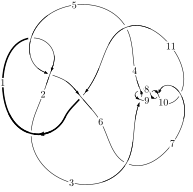
\includegraphics[width=112pt]{../../../GIT/diagram.site/Diagrams/png/333_11a_84.png}\\
\ \ \ A knot diagram\footnotemark}&
\allowdisplaybreaks
\textbf{Linearized knot diagam} \\
\cline{2-2}
 &
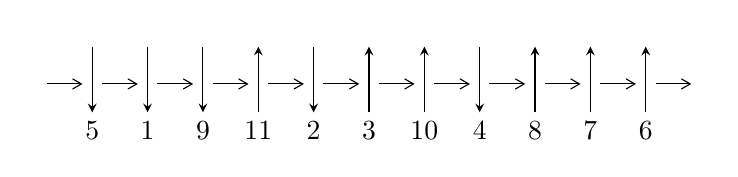
\begin{tikzpicture}[x=20pt, y=17pt]
	% nodes
	\node (C0) at (0, 0) {};
	\node (C1) at (1, 0) {};
	\node (C1U) at (1, +1) {};
	\node (C1D) at (1, -1) {5};

	\node (C2) at (2, 0) {};
	\node (C2U) at (2, +1) {};
	\node (C2D) at (2, -1) {1};

	\node (C3) at (3, 0) {};
	\node (C3U) at (3, +1) {};
	\node (C3D) at (3, -1) {9};

	\node (C4) at (4, 0) {};
	\node (C4U) at (4, +1) {};
	\node (C4D) at (4, -1) {11};

	\node (C5) at (5, 0) {};
	\node (C5U) at (5, +1) {};
	\node (C5D) at (5, -1) {2};

	\node (C6) at (6, 0) {};
	\node (C6U) at (6, +1) {};
	\node (C6D) at (6, -1) {3};

	\node (C7) at (7, 0) {};
	\node (C7U) at (7, +1) {};
	\node (C7D) at (7, -1) {10};

	\node (C8) at (8, 0) {};
	\node (C8U) at (8, +1) {};
	\node (C8D) at (8, -1) {4};

	\node (C9) at (9, 0) {};
	\node (C9U) at (9, +1) {};
	\node (C9D) at (9, -1) {8};

	\node (C10) at (10, 0) {};
	\node (C10U) at (10, +1) {};
	\node (C10D) at (10, -1) {7};

	\node (C11) at (11, 0) {};
	\node (C11U) at (11, +1) {};
	\node (C11D) at (11, -1) {6};
	\node (C12) at (12, 0) {};

	% arrows
	\draw[->,>={angle 60}]
	(C0) edge (C1) (C1) edge (C2) (C2) edge (C3) (C3) edge (C4) (C4) edge (C5) (C5) edge (C6) (C6) edge (C7) (C7) edge (C8) (C8) edge (C9) (C9) edge (C10) (C10) edge (C11) (C11) edge (C12) ;	\draw[->,>=stealth]
	(C1U) edge (C1D) (C2U) edge (C2D) (C3U) edge (C3D) (C4D) edge (C4U) (C5U) edge (C5D) (C6D) edge (C6U) (C7D) edge (C7U) (C8U) edge (C8D) (C9D) edge (C9U) (C10D) edge (C10U) (C11D) edge (C11U) ;
	\end{tikzpicture} \\
\hhline{~~} \\& 
\textbf{Solving Sequence} \\ \cline{2-2} 
 &
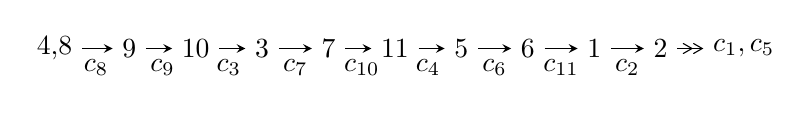
\begin{tikzpicture}[x=24pt, y=7pt]
	% node
	\node (A0) at (-1/8, 0) {4,8};
	\node (A1) at (1, 0) {9};
	\node (A2) at (2, 0) {10};
	\node (A3) at (3, 0) {3};
	\node (A4) at (4, 0) {7};
	\node (A5) at (5, 0) {11};
	\node (A6) at (6, 0) {5};
	\node (A7) at (7, 0) {6};
	\node (A8) at (8, 0) {1};
	\node (A9) at (9, 0) {2};
	\node (C1) at (1/2, -1) {$c_{8}$};
	\node (C2) at (3/2, -1) {$c_{9}$};
	\node (C3) at (5/2, -1) {$c_{3}$};
	\node (C4) at (7/2, -1) {$c_{7}$};
	\node (C5) at (9/2, -1) {$c_{10}$};
	\node (C6) at (11/2, -1) {$c_{4}$};
	\node (C7) at (13/2, -1) {$c_{6}$};
	\node (C8) at (15/2, -1) {$c_{11}$};
	\node (C9) at (17/2, -1) {$c_{2}$};
	\node (A10) at (41/4, 0) {$c_{1},c_{5}$};

	% edge
	\draw[->,>=stealth]	
	(A0) edge (A1) (A1) edge (A2) (A2) edge (A3) (A3) edge (A4) (A4) edge (A5) (A5) edge (A6) (A6) edge (A7) (A7) edge (A8) (A8) edge (A9) ;
	\draw[->>,>={angle 60}]	
	(A9) edge (A10);
\end{tikzpicture} \\ 

\end{tabular} \\

\footnotetext{
The image of knot diagram is generated by the software ``\textbf{Draw programme}" developed by Andrew Bartholomew(\url{http://www.layer8.co.uk/maths/draw/index.htm\#Running-draw}), where we modified some parts for our purpose(\url{https://github.com/CATsTAILs/LinksPainter}).
}\phantom \\ \newline 
\centering \textbf{Ideals for irreducible components\footnotemark of $X_{\text{par}}$} 
 
\begin{align*}
I^u_{1}&=\langle 
u^{50}+u^{49}+\cdots- u+1\rangle \\
\\
\end{align*}
\raggedright * 1 irreducible components of $\dim_{\mathbb{C}}=0$, with total 50 representations.\\
\footnotetext{All coefficients of polynomials are rational numbers. But the coefficients are sometimes approximated in decimal forms when there is not enough margin.}
\newpage
\renewcommand{\arraystretch}{1}
\centering \section*{I. $I^u_{1}= \langle u^{50}+u^{49}+\cdots- u+1 \rangle$}
\flushleft \textbf{(i) Arc colorings}\\
\begin{tabular}{m{7pt} m{180pt} m{7pt} m{180pt} }
\flushright $a_{4}=$&$\begin{pmatrix}0\\u\end{pmatrix}$ \\
\flushright $a_{8}=$&$\begin{pmatrix}1\\0\end{pmatrix}$ \\
\flushright $a_{9}=$&$\begin{pmatrix}1\\u^2\end{pmatrix}$ \\
\flushright $a_{10}=$&$\begin{pmatrix}u^2+1\\u^2\end{pmatrix}$ \\
\flushright $a_{3}=$&$\begin{pmatrix}u\\u^3+u\end{pmatrix}$ \\
\flushright $a_{7}=$&$\begin{pmatrix}u^4+u^2+1\\u^4\end{pmatrix}$ \\
\flushright $a_{11}=$&$\begin{pmatrix}u^6+u^4+2 u^2+1\\u^6+u^2\end{pmatrix}$ \\
\flushright $a_{5}=$&$\begin{pmatrix}u^{13}+2 u^{11}+5 u^9+6 u^7+6 u^5+4 u^3+u\\u^{13}+u^{11}+3 u^9+2 u^7+2 u^5+u^3+u\end{pmatrix}$ \\
\flushright $a_{6}=$&$\begin{pmatrix}u^8+u^6+3 u^4+2 u^2+1\\u^{10}+2 u^8+3 u^6+4 u^4+u^2\end{pmatrix}$ \\
\flushright $a_{1}=$&$\begin{pmatrix}- u^{24}-3 u^{22}+\cdots+2 u^2+1\\- u^{26}-4 u^{24}+\cdots-3 u^6+u^2\end{pmatrix}$ \\
\flushright $a_{2}=$&$\begin{pmatrix}u^{47}+6 u^{45}+\cdots+4 u^3+2 u\\u^{49}+7 u^{47}+\cdots+2 u^3+u\end{pmatrix}$\\ \flushright $a_{2}=$&$\begin{pmatrix}u^{47}+6 u^{45}+\cdots+4 u^3+2 u\\u^{49}+7 u^{47}+\cdots+2 u^3+u\end{pmatrix}$\\&\end{tabular}
\flushleft \textbf{(ii) Obstruction class $= -1$}\\~\\
\flushleft \textbf{(iii) Cusp Shapes $= 4 u^{48}+4 u^{47}+\cdots-20 u^3-2$}\\~\\
\newpage\renewcommand{\arraystretch}{1}
\flushleft \textbf{(iv) u-Polynomials at the component}\newline \\
\begin{tabular}{m{50pt}|m{274pt}}
Crossings & \hspace{64pt}u-Polynomials at each crossing \\
\hline $$\begin{aligned}c_{1},c_{5}\end{aligned}$$&$\begin{aligned}
&u^{50}+u^{49}+\cdots- u+1
\end{aligned}$\\
\hline $$\begin{aligned}c_{2}\end{aligned}$$&$\begin{aligned}
&u^{50}+23 u^{49}+\cdots- u+1
\end{aligned}$\\
\hline $$\begin{aligned}c_{3},c_{8}\end{aligned}$$&$\begin{aligned}
&u^{50}- u^{49}+\cdots+u+1
\end{aligned}$\\
\hline $$\begin{aligned}c_{4},c_{6}\end{aligned}$$&$\begin{aligned}
&u^{50}- u^{49}+\cdots-165 u+25
\end{aligned}$\\
\hline $$\begin{aligned}c_{7},c_{9},c_{10}\end{aligned}$$&$\begin{aligned}
&u^{50}-13 u^{49}+\cdots- u+1
\end{aligned}$\\
\hline $$\begin{aligned}c_{11}\end{aligned}$$&$\begin{aligned}
&u^{50}+3 u^{49}+\cdots+u+3
\end{aligned}$\\
\hline
\end{tabular}\\~\\
\newpage\renewcommand{\arraystretch}{1}
\flushleft \textbf{(v) Riley Polynomials at the component}\newline \\
\begin{tabular}{m{50pt}|m{274pt}}
Crossings & \hspace{64pt}Riley Polynomials at each crossing \\
\hline $$\begin{aligned}c_{1},c_{5}\end{aligned}$$&$\begin{aligned}
&y^{50}-23 y^{49}+\cdots+y+1
\end{aligned}$\\
\hline $$\begin{aligned}c_{2}\end{aligned}$$&$\begin{aligned}
&y^{50}+9 y^{49}+\cdots+y+1
\end{aligned}$\\
\hline $$\begin{aligned}c_{3},c_{8}\end{aligned}$$&$\begin{aligned}
&y^{50}+13 y^{49}+\cdots+y+1
\end{aligned}$\\
\hline $$\begin{aligned}c_{4},c_{6}\end{aligned}$$&$\begin{aligned}
&y^{50}-31 y^{49}+\cdots-16275 y+625
\end{aligned}$\\
\hline $$\begin{aligned}c_{7},c_{9},c_{10}\end{aligned}$$&$\begin{aligned}
&y^{50}+49 y^{49}+\cdots-7 y+1
\end{aligned}$\\
\hline $$\begin{aligned}c_{11}\end{aligned}$$&$\begin{aligned}
&y^{50}+5 y^{49}+\cdots+521 y+9
\end{aligned}$\\
\hline
\end{tabular}\\~\\
\newpage\flushleft \textbf{(vi) Complex Volumes and Cusp Shapes}
$$\begin{array}{c|c|c}  
\text{Solutions to }I^u_{1}& \I (\text{vol} + \sqrt{-1}CS) & \text{Cusp shape}\\
 \hline 
\begin{aligned}
u &= \phantom{-}0.219529 + 0.986047 I\end{aligned}
 & \phantom{-}3.94354 + 3.43046 I & \phantom{-}5.76669 - 1.67529 I \\ \hline\begin{aligned}
u &= \phantom{-}0.219529 - 0.986047 I\end{aligned}
 & \phantom{-}3.94354 - 3.43046 I & \phantom{-}5.76669 + 1.67529 I \\ \hline\begin{aligned}
u &= -0.246085 + 0.982711 I\end{aligned}
 & \phantom{-}5.58031 + 1.62349 I & \phantom{-}8.34360 - 3.64621 I \\ \hline\begin{aligned}
u &= -0.246085 - 0.982711 I\end{aligned}
 & \phantom{-}5.58031 - 1.62349 I & \phantom{-}8.34360 + 3.64621 I \\ \hline\begin{aligned}
u &= \phantom{-}0.308256 + 0.923731 I\end{aligned}
 & \phantom{-}0.40552 - 2.46934 I & \phantom{-}0.87793 + 4.65157 I \\ \hline\begin{aligned}
u &= \phantom{-}0.308256 - 0.923731 I\end{aligned}
 & \phantom{-}0.40552 + 2.46934 I & \phantom{-}0.87793 - 4.65157 I \\ \hline\begin{aligned}
u &= -0.298826 + 0.987833 I\end{aligned}
 & \phantom{-}5.26972 + 4.23270 I & \phantom{-}7.37704 - 4.53289 I \\ \hline\begin{aligned}
u &= -0.298826 - 0.987833 I\end{aligned}
 & \phantom{-}5.26972 - 4.23270 I & \phantom{-}7.37704 + 4.53289 I \\ \hline\begin{aligned}
u &= \phantom{-}0.318075 + 0.994530 I\end{aligned}
 & \phantom{-}3.36572 - 9.34553 I & \phantom{-}4.11417 + 9.06753 I \\ \hline\begin{aligned}
u &= \phantom{-}0.318075 - 0.994530 I\end{aligned}
 & \phantom{-}3.36572 + 9.34553 I & \phantom{-}4.11417 - 9.06753 I \\ \hline\begin{aligned}
u &= -0.775854 + 0.801832 I\end{aligned}
 & -2.39389 + 4.71062 I & -0.14636 - 5.46565 I \\ \hline\begin{aligned}
u &= -0.775854 - 0.801832 I\end{aligned}
 & -2.39389 - 4.71062 I & -0.14636 + 5.46565 I \\ \hline\begin{aligned}
u &= -0.483537 + 0.734912 I\end{aligned}
 & -1.95260 + 5.09579 I & -2.40884 - 8.50757 I \\ \hline\begin{aligned}
u &= -0.483537 - 0.734912 I\end{aligned}
 & -1.95260 - 5.09579 I & -2.40884 + 8.50757 I \\ \hline\begin{aligned}
u &= \phantom{-}0.811513 + 0.797475 I\end{aligned}
 & -1.169710 + 0.163979 I & \phantom{-}1.95677 - 0.52892 I \\ \hline\begin{aligned}
u &= \phantom{-}0.811513 - 0.797475 I\end{aligned}
 & -1.169710 - 0.163979 I & \phantom{-}1.95677 + 0.52892 I \\ \hline\begin{aligned}
u &= \phantom{-}0.852019 + 0.801997 I\end{aligned}
 & -2.15185 + 2.58590 I & \phantom{-}0.827994 - 0.674583 I \\ \hline\begin{aligned}
u &= \phantom{-}0.852019 - 0.801997 I\end{aligned}
 & -2.15185 - 2.58590 I & \phantom{-}0.827994 + 0.674583 I \\ \hline\begin{aligned}
u &= \phantom{-}0.085415 + 0.824761 I\end{aligned}
 & \phantom{-}1.16249 - 1.82384 I & \phantom{-}6.57065 + 4.44419 I \\ \hline\begin{aligned}
u &= \phantom{-}0.085415 - 0.824761 I\end{aligned}
 & \phantom{-}1.16249 + 1.82384 I & \phantom{-}6.57065 - 4.44419 I \\ \hline\begin{aligned}
u &= -0.863831 + 0.802647 I\end{aligned}
 & -4.29327 - 7.68607 I & -2.29729 + 4.73536 I \\ \hline\begin{aligned}
u &= -0.863831 - 0.802647 I\end{aligned}
 & -4.29327 + 7.68607 I & -2.29729 - 4.73536 I \\ \hline\begin{aligned}
u &= -0.850278 + 0.827510 I\end{aligned}
 & -6.91480 - 0.19952 I & -5.59281 + 0. I\phantom{ +0.000000I} \\ \hline\begin{aligned}
u &= -0.850278 - 0.827510 I\end{aligned}
 & -6.91480 + 0.19952 I & -5.59281 + 0. I\phantom{ +0.000000I} \\ \hline\begin{aligned}
u &= -0.757117 + 0.952106 I\end{aligned}
 & -1.93934 + 1.09281 I & \phantom{-0.000000 } 0 \\ \hline\begin{aligned}
u &= -0.757117 - 0.952106 I\end{aligned}
 & -1.93934 - 1.09281 I & \phantom{-0.000000 } 0 \\ \hline\begin{aligned}
u &= -0.825284 + 0.899193 I\end{aligned}
 & -6.17694 + 3.07827 I & \phantom{-0.000000 } 0. - 2.72625 I \\ \hline\begin{aligned}
u &= -0.825284 - 0.899193 I\end{aligned}
 & -6.17694 - 3.07827 I & \phantom{-0.000000 -}0. + 2.72625 I \\ \hline\begin{aligned}
u &= \phantom{-}0.845830 + 0.890740 I\end{aligned}
 & -9.32972 + 0.72052 I & -6.40734 + 0. I\phantom{ +0.000000I} \\ \hline\begin{aligned}
u &= \phantom{-}0.845830 - 0.890740 I\end{aligned}
 & -9.32972 - 0.72052 I & -6.40734 + 0. I\phantom{ +0.000000I}\\
 \hline 
 \end{array}$$\newpage$$\begin{array}{c|c|c}  
\text{Solutions to }I^u_{1}& \I (\text{vol} + \sqrt{-1}CS) & \text{Cusp shape}\\
 \hline 
\begin{aligned}
u &= \phantom{-}0.771222 + 0.962943 I\end{aligned}
 & -0.66571 - 6.10737 I & \phantom{-0.000000 -}0. + 5.65000 I \\ \hline\begin{aligned}
u &= \phantom{-}0.771222 - 0.962943 I\end{aligned}
 & -0.66571 + 6.10737 I & \phantom{-0.000000 } 0. - 5.65000 I \\ \hline\begin{aligned}
u &= \phantom{-}0.836263 + 0.917270 I\end{aligned}
 & -9.24690 - 6.97433 I & -6.10425 + 6.45667 I \\ \hline\begin{aligned}
u &= \phantom{-}0.836263 - 0.917270 I\end{aligned}
 & -9.24690 + 6.97433 I & -6.10425 - 6.45667 I \\ \hline\begin{aligned}
u &= \phantom{-}0.332618 + 0.672808 I\end{aligned}
 & \phantom{-}0.174284 - 1.327380 I & \phantom{-}1.54374 + 5.34383 I \\ \hline\begin{aligned}
u &= \phantom{-}0.332618 - 0.672808 I\end{aligned}
 & \phantom{-}0.174284 + 1.327380 I & \phantom{-}1.54374 - 5.34383 I \\ \hline\begin{aligned}
u &= -0.802884 + 0.962136 I\end{aligned}
 & -6.49492 + 6.35925 I & \phantom{-0.000000 } 0 \\ \hline\begin{aligned}
u &= -0.802884 - 0.962136 I\end{aligned}
 & -6.49492 - 6.35925 I & \phantom{-0.000000 } 0 \\ \hline\begin{aligned}
u &= \phantom{-}0.792536 + 0.977055 I\end{aligned}
 & -1.60913 - 8.71493 I & \phantom{-0.000000 } 0 \\ \hline\begin{aligned}
u &= \phantom{-}0.792536 - 0.977055 I\end{aligned}
 & -1.60913 + 8.71493 I & \phantom{-0.000000 } 0 \\ \hline\begin{aligned}
u &= -0.798650 + 0.982182 I\end{aligned}
 & -3.7340 + 13.8696 I & \phantom{-0.000000 } 0. - 9.53503 I \\ \hline\begin{aligned}
u &= -0.798650 - 0.982182 I\end{aligned}
 & -3.7340 - 13.8696 I & \phantom{-0.000000 -}0. + 9.53503 I \\ \hline\begin{aligned}
u &= -0.488576 + 0.512324 I\end{aligned}
 & -2.60376 - 1.44363 I & -5.78396 + 0.53575 I \\ \hline\begin{aligned}
u &= -0.488576 - 0.512324 I\end{aligned}
 & -2.60376 + 1.44363 I & -5.78396 - 0.53575 I \\ \hline\begin{aligned}
u &= \phantom{-}0.630218 + 0.101743 I\end{aligned}
 & \phantom{-}0.59402 + 6.02058 I & -1.82523 - 5.20463 I \\ \hline\begin{aligned}
u &= \phantom{-}0.630218 - 0.101743 I\end{aligned}
 & \phantom{-}0.59402 - 6.02058 I & -1.82523 + 5.20463 I \\ \hline\begin{aligned}
u &= -0.605378 + 0.059120 I\end{aligned}
 & \phantom{-}2.43882 - 1.09952 I & \phantom{-}1.50149 + 0.50378 I \\ \hline\begin{aligned}
u &= -0.605378 - 0.059120 I\end{aligned}
 & \phantom{-}2.43882 + 1.09952 I & \phantom{-}1.50149 - 0.50378 I \\ \hline\begin{aligned}
u &= \phantom{-}0.492805 + 0.206145 I\end{aligned}
 & -1.73630 - 0.52214 I & -5.82516 + 0.81274 I \\ \hline\begin{aligned}
u &= \phantom{-}0.492805 - 0.206145 I\end{aligned}
 & -1.73630 + 0.52214 I & -5.82516 - 0.81274 I\\
 \hline 
 \end{array}$$\newpage
\newpage\renewcommand{\arraystretch}{1}
\centering \section*{ II. u-Polynomials}
\begin{tabular}{m{50pt}|m{274pt}}
Crossings & \hspace{64pt}u-Polynomials at each crossing \\
\hline $$\begin{aligned}c_{1},c_{5}\end{aligned}$$&$\begin{aligned}
&u^{50}+u^{49}+\cdots- u+1
\end{aligned}$\\
\hline $$\begin{aligned}c_{2}\end{aligned}$$&$\begin{aligned}
&u^{50}+23 u^{49}+\cdots- u+1
\end{aligned}$\\
\hline $$\begin{aligned}c_{3},c_{8}\end{aligned}$$&$\begin{aligned}
&u^{50}- u^{49}+\cdots+u+1
\end{aligned}$\\
\hline $$\begin{aligned}c_{4},c_{6}\end{aligned}$$&$\begin{aligned}
&u^{50}- u^{49}+\cdots-165 u+25
\end{aligned}$\\
\hline $$\begin{aligned}c_{7},c_{9},c_{10}\end{aligned}$$&$\begin{aligned}
&u^{50}-13 u^{49}+\cdots- u+1
\end{aligned}$\\
\hline $$\begin{aligned}c_{11}\end{aligned}$$&$\begin{aligned}
&u^{50}+3 u^{49}+\cdots+u+3
\end{aligned}$\\
\hline
\end{tabular}\newpage\renewcommand{\arraystretch}{1}
\centering \section*{ III. Riley Polynomials}
\begin{tabular}{m{50pt}|m{274pt}}
Crossings & \hspace{64pt}Riley Polynomials at each crossing \\
\hline $$\begin{aligned}c_{1},c_{5}\end{aligned}$$&$\begin{aligned}
&y^{50}-23 y^{49}+\cdots+y+1
\end{aligned}$\\
\hline $$\begin{aligned}c_{2}\end{aligned}$$&$\begin{aligned}
&y^{50}+9 y^{49}+\cdots+y+1
\end{aligned}$\\
\hline $$\begin{aligned}c_{3},c_{8}\end{aligned}$$&$\begin{aligned}
&y^{50}+13 y^{49}+\cdots+y+1
\end{aligned}$\\
\hline $$\begin{aligned}c_{4},c_{6}\end{aligned}$$&$\begin{aligned}
&y^{50}-31 y^{49}+\cdots-16275 y+625
\end{aligned}$\\
\hline $$\begin{aligned}c_{7},c_{9},c_{10}\end{aligned}$$&$\begin{aligned}
&y^{50}+49 y^{49}+\cdots-7 y+1
\end{aligned}$\\
\hline $$\begin{aligned}c_{11}\end{aligned}$$&$\begin{aligned}
&y^{50}+5 y^{49}+\cdots+521 y+9
\end{aligned}$\\
\hline
\end{tabular}
\vskip 2pc
\end{document}